%--------------------------------------------%
% Template Beamer para Apresentações da UFRN %
% by alcemygvseverino@gmail.com              %
% Baseado em MIT Beamer Template			 %
% versao 1.1								 %
% Atualizado em 14/05/2016					 %
%--------------------------------------------%
\documentclass[handout,t]{beamer}
% Para alterar a linguagem do documento
\usepackage[english]{babel}
% Para aceitar caracteres especias deretamente do teclado
\usepackage[utf8]{inputenc}
% Para seguir as normas da ABNT de citacao e referencias
\usepackage[alf]{abntex2cite}
% To include figures
\usepackage{graphicx}
% Para melhor ajuste da posisao das figuras
\usepackage{float}
\usepackage{geometry}
\usepackage{amsmath}
\usepackage{amssymb}
\usepackage{url}
% Para incluir paginas de documentos .pdf externos
\usepackage{pgfpages}
\usepackage{pgf}
% Para ajustar o estilo dos contadores
\usepackage{enumerate}
% Para modificar a cor do texto
\usepackage{color}
% Para incluir condicoes
\usepackage{ifthen}
% Para colocar legendas em algo que nao e float
\usepackage{capt-of}
% Para definir o tema do slide
\usetheme{Berlin}
% Para difinir cores e background
\usecolortheme{ufrn}
% Para numerar as figuras
\setbeamertemplate{caption}[numbered]
% For hyperlinks
\usepackage{hyperref}

% Title
\title[Princeton Group Meeting]{
	Princeton Weekly Group Meeting: \\ Slides}
% Data
\date{July 11, 2019}
% Authors
\author[Stephanie Kwan]{
	Stephanie Kwan \\
	\textrm{skwan@princeton.edu} %\inst{1}
%	\\	\vspace{0.25cm}
%	Autor 02 \inst{2}
}



% Institution
\institute[Institutions]{
%	\inst{1}%
	Princeton University}
% Right bottom corner



\logo{
\includegraphics[width=.05\textwidth]{figures/Princetonshieldlarge.png}~~%
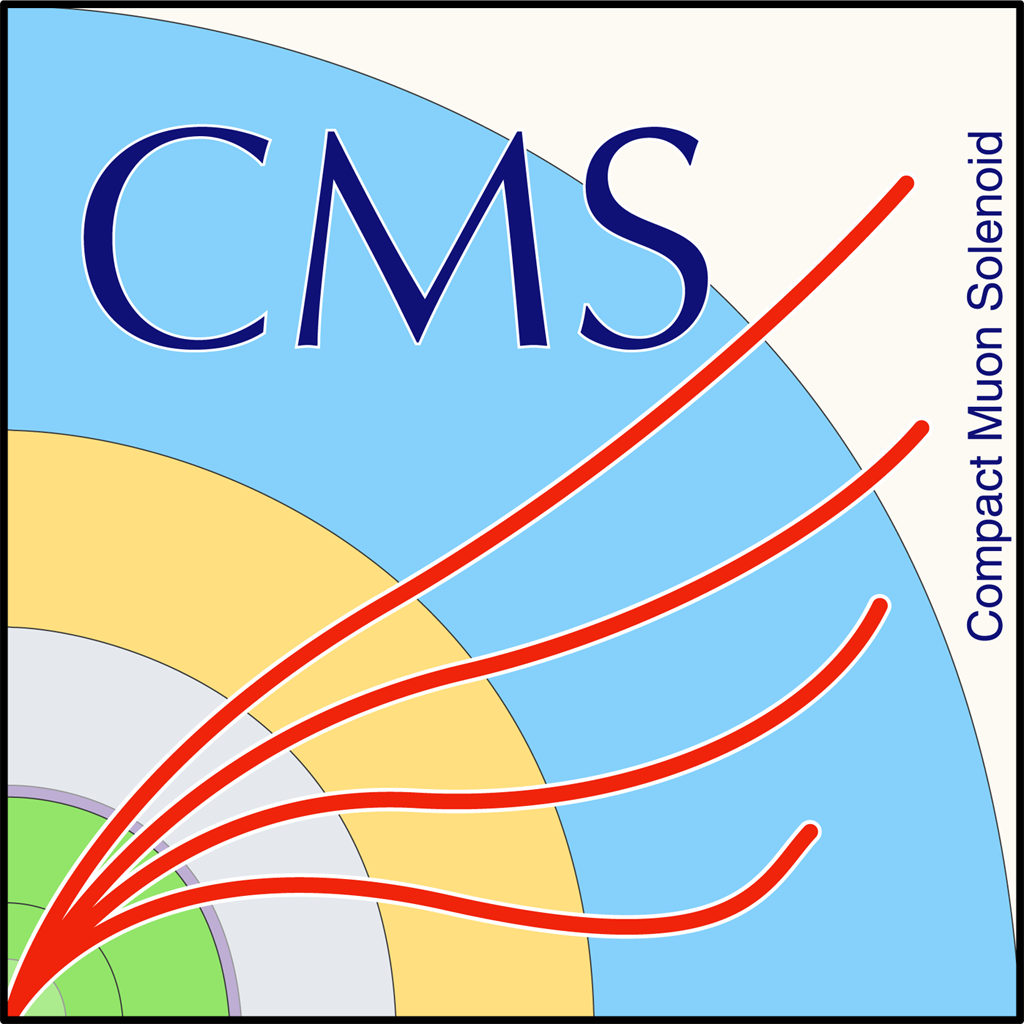
\includegraphics[width=.06\textwidth]{figures/CMSlogo.png}}



\begin{document}
% Summary
    
\frame{\titlepage}
\section[]{}
\begin{frame}{Summary}
	\tableofcontents
\end{frame}

% Introduction
\section{Introduction}
\begin{frame}{Title}

\end{frame}


\begin{frame}{Title 2}
    \begin{figure}\vspace{-0.3cm}
            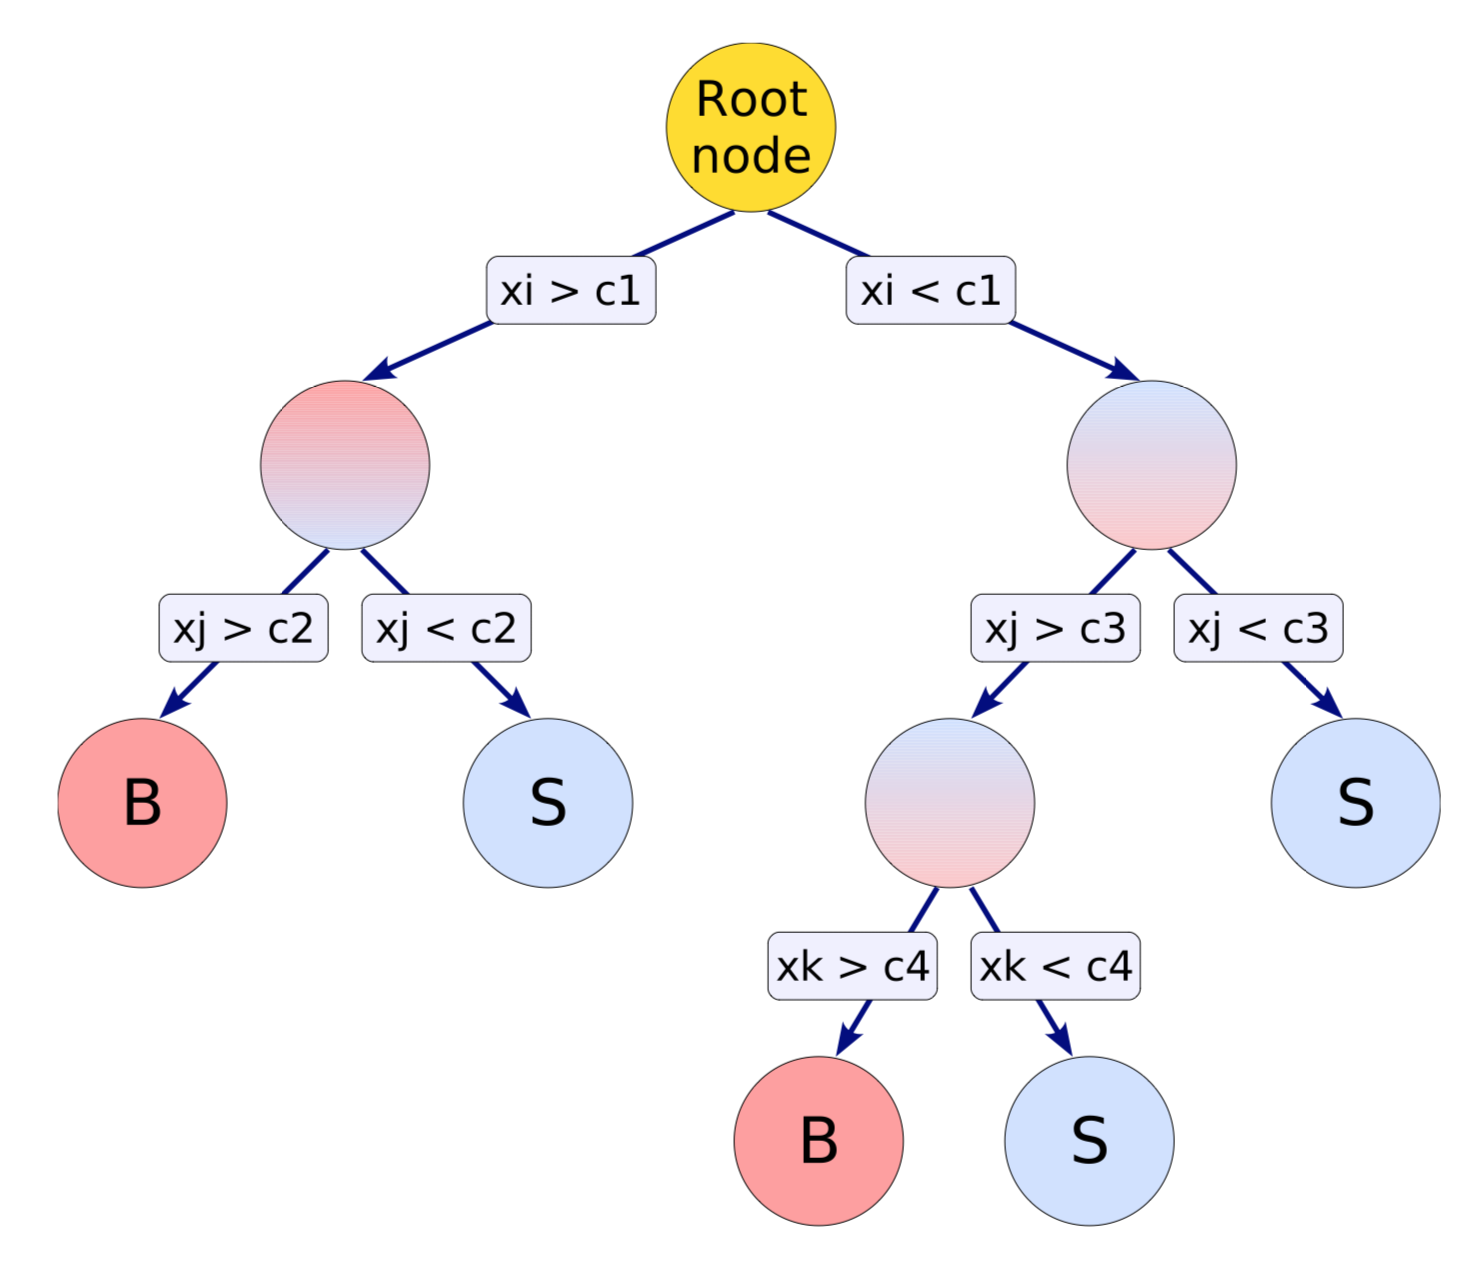
\includegraphics[width=0.55\textwidth]{figures/bdt_example_from_TMVA_handbook.png}
            \caption{Caption}
        \end{figure}
\end{frame}

% Methodology
\section{Methodology}

\begin{frame}{Title}
    \label{Title_label}\vspace{-0.5cm}\hspace{-2cm}
     
\end{frame}

\begin{frame}{Page with columns}
    
	\begin{columns}
	\begin{column}{0.5\textwidth}
	    \begin{figure}\vspace{-0.7cm}
            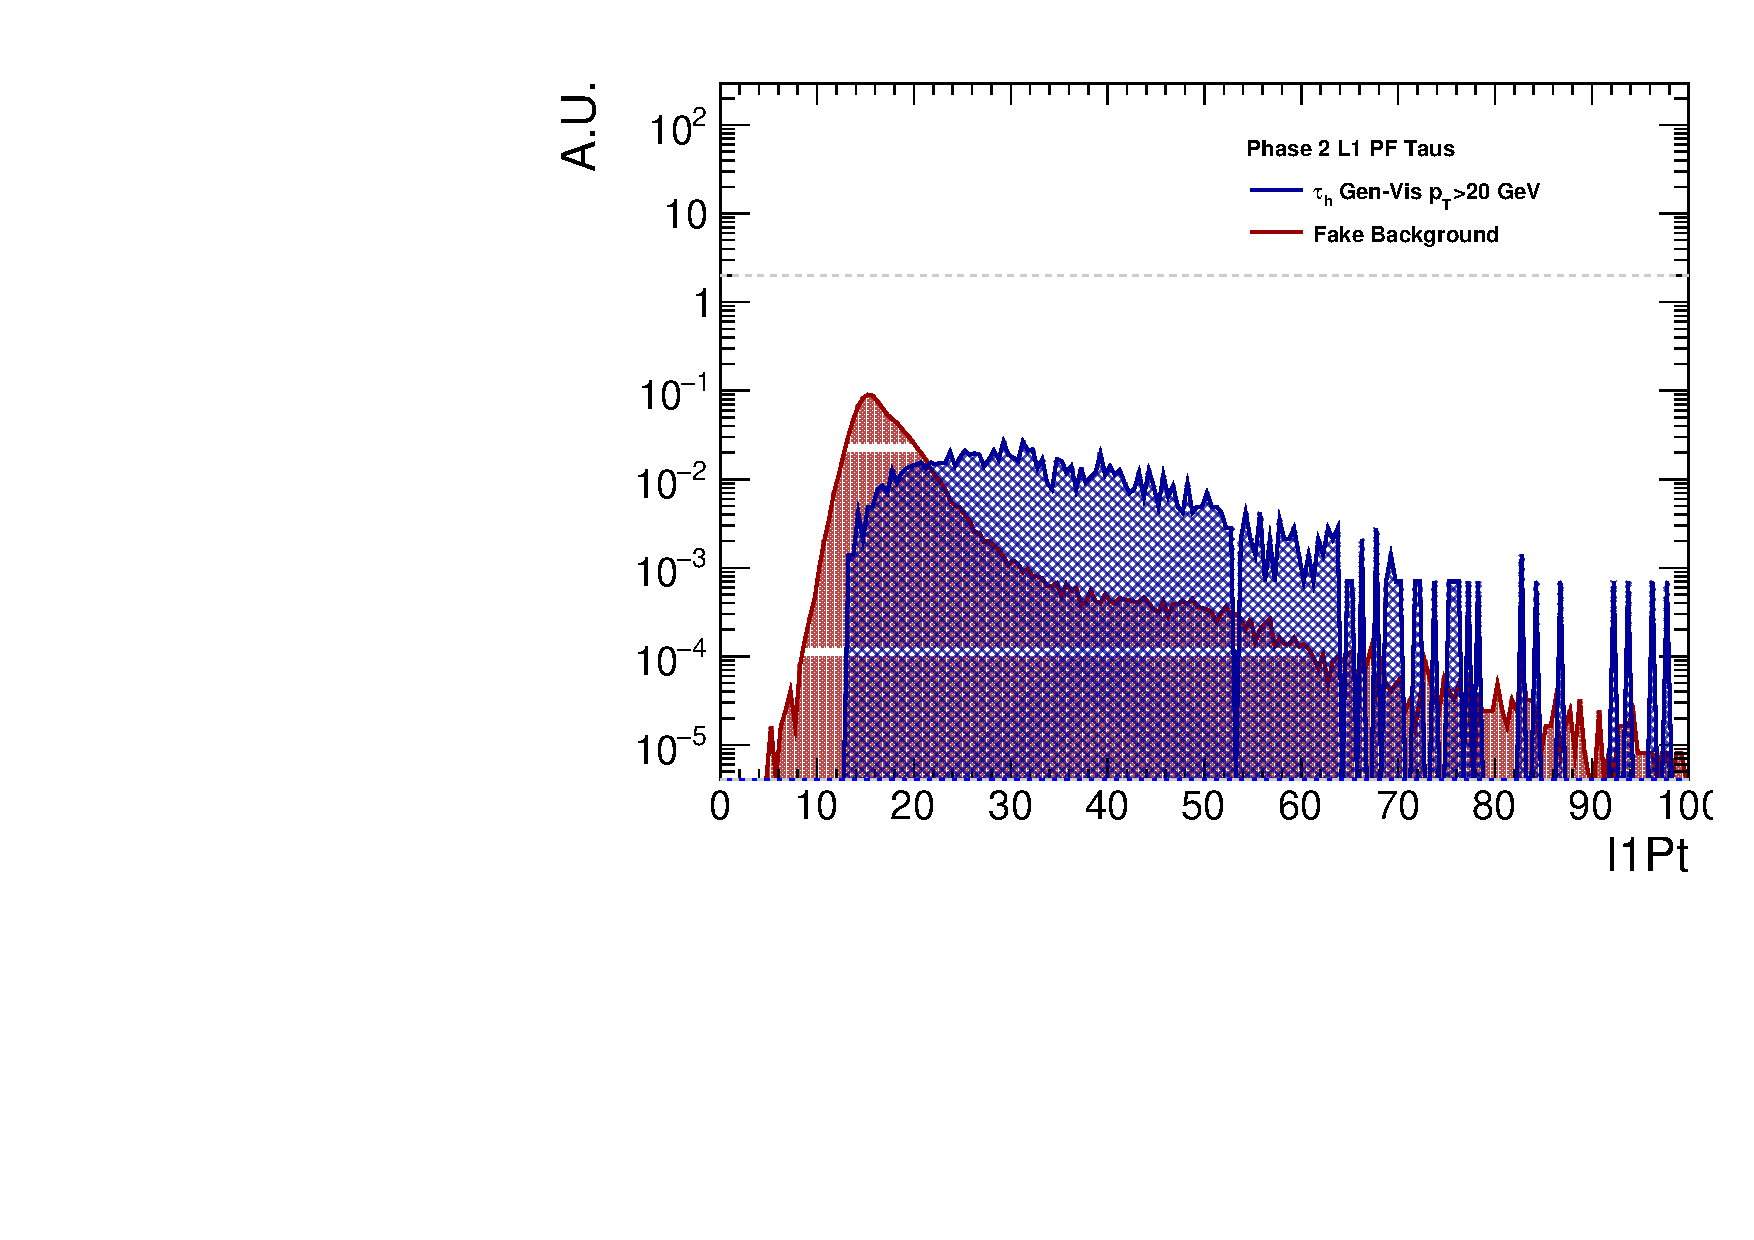
\includegraphics[width=1.0\textwidth]{figures/dyll_l1Pt.pdf}
            \caption{Input 1 of 5: l1Pt signal (blue) vs background (red).}
            
        \end{figure}
	\end{column}
	\begin{column}{0.5\textwidth}
        Column text here
    \end{column}
    \end{columns}
    
\end{frame}



% Results
\section{Conclusion}
\begin{frame}{Conclusion}\vspace*{-0.3cm}
\end{frame}


% Conclusion
\include{tex/conclusion/conclusion}

% Backup slides
\section{}

\appendix

\begin{frame}{Backup slides:}
    Backup slides go here.
\end{frame}

% References
%%\section{References}
\begin{frame}{References}
	\bibliography{bib/bibliografia}
\end{frame}

% Acknowledgments
%\section{}
%\begin{frame}{Acknowledgments}
%	Agradeço a todos. 	
%\end{frame}

\end{document}